\chapter{Reactor Model} \label{ch:mass_model}
The reactor mass model was created as a submodel of the power cycle mass
model. The reactor mass model was designed to take flow property inputs (T, P,
$\dot{m}$) and constrain a reactor concept that was both coolable, and critical
after 10 years of full power operation. The reactor model was developed in
Python. The attribute of interest was the mass of
the valid concept, but other useful values such as geometry, fuel fraction,
and fluid-flow paramters were available from the solver. Before the mass model
could be built, some important design decisions needed to be made.

\section{Thermal Hydraulic Model}
The second considered constraint of a valid reactor design was coolability. The reactor must
not melt and the integrity of the fuel must be maintained for the duration of
the mission. To ensure the thermal hydraulic validity of a chosen design, 
1D heat transfer and bulk-averaged fluid flow calculations were performed. The 1D
heat transfer and fluid equations were coupled with analytical peaking factors
factors from nuclear engineering literature to determine the maximum extractable
thermal power for each reactor design. A 1D resistance network was used to
determine the maximum thermal generation for a given core design and a temperature
drop between fuel and coolant. An iterative solving scheme was developed to
converge the heat transfer and fluid flow equations.

\subsection{Flow Properties}
All flow properties were axially averaged between their inlet and outlet values.
The inlet and outlet flow conditions, thermal power, and mass flow rate were
dictated by the power cycle configuration and requirements. Property tables for
both CO2 and H2O coolants as a function of pressure and temperature were 
generated using EES and interpolated using SciPy's 2D interpolation functions
\citep{scipy}, \citep{EES_citation}.
The interpolated properties included: thermal conductivity [$\frac{W}{m-K}$], density
[$\frac{kg}{m^3}$], viscosity [$\frac{kg}{m-s}$], and specific heat [$\frac{kJ}{kg-K}$].

\subsection{Thermophysical Properties}
Thermophysical properties were used to model heat transfer in solid reactor
components. Thermal conductivity was required for conduction, density was
required for mass calculations, cladding roughness was required for Nusselt
numbers, and material strength was required for pressure vessel thickness.
Material densities are shown in Table \ref{tab:densities}.

\begin{table}[h]
  \centering
  \caption{Solid Material Densities}
  \begin{tabular}{lll}
    \toprule
     Material        & Density  [$\frac{kg}{m^3}$]     \\ 
    \midrule                                  
     Uranium Nitride & 11,300 \\
     Uranium Oxide   & 10,940 \\
     Tungsten        & 19,300 \\
     Inconel-718     & 8,190  \\
     Graphite        & 1,700  \\
     SS-304          & 8,050
  \end{tabular}
  \label{tab:densities}
\end{table}

The fuel density of the UW-CERMET cores was calculated assuming 60\% UN fuel and
40\% tungsten matrix by volume \citep{conduct_cermet}. Thermal conductivity was
used for conduction in the fuel and cladding. The CERMET conductivity was a
combination of the conductivity of UN and W \citep{conduct_cermet}, conductivity
in the CERMET fuel was 51 $[\frac{W}/{m-K}]$. The \uox thermal conductivity used
was 3.6 $[\frac{W}/{m-K}]$ \citep{todreas_th}. The yield strength for SS-304 was
used to calculate the required pressure vessel thicknes, the yield strength for
SS-304 was 275 [MPa] \citep{ss_strength}.

\subsection{Calculation Overview}
The thermal hydraulic mass calculation was broken down into a series of steps.
\begin{enumerate}
    \item Core geometry
    \item Flow characterization
    \item 1D heat transfer
    \item Pressure check and mass calculations
\end{enumerate}

\subsection{Core Geometry}
Important core geometry parameters were calculated. The coolant flow area,
average distance of conduction in the fuel, volume fraction of cladding in
coolant, number of coolant channels, convection surface area, LD, and the cross
sectional area for conduction in the fuel were all defined in this step. The
core radius is set by the critical
radius constraint dependent on the fuel fraction.

Fuel area and volume was derived from the core radius and fuel fraction (f). Where
$AR$ was the core aspect ratio.

\begin{equation}
    A_{fuel} = f_{fuel}\cdot r_{core}^2 \cdot \pi
\end{equation}
\begin{equation}
    V_{fuel} = A_{fuel}\cdot AR\cdot r_{core}
\end{equation}

The fraction of cladding in the coolant was derived from the coolant channel
radius and cladding thickness.

\begin{equation}
    f_{clad} = \frac{(r_{channel} + t_{clad})^2}{r_{channel}^2} - 1 
\end{equation}

In a similar vein, coolant flow area was derived from the core radius, cladding
fraction, and fuel fraction

\begin{equation}
    A_{cool} = (1-frac_{fuel})\cdot (1-frac_{clad}) \cdot r_{core}^2 \cdot \pi
\end{equation}

\begin{equation}
    V_{cool} = A_{cool}\cdot AR\cdot r_{core}
\end{equation}

The number of coolant channels was derived from the area of each channel and the
core flow area.

\begin{equation}
    N_{channels} = \frac{A_{cool}}{(r_{channel} + t_{clad})^2 \cdot \pi}
\end{equation}

The convection surface area was dervied from the channel radius, core length, and
number of channels (N).

\begin{equation}
    A_{conv} = 2\cdot r_{channel}\cdot \pi\cdot r_{core}\cdot AR\cdot N
\end{equation}

The length over diameter was derived from the channel radius and core length.

\begin{equation}
    LD = \frac{r_{core}\cdot AR}{2\cdot r_{channel}}
\end{equation}

The average distance to conduction was derived from fuel area and number of
channels assuming a square unit cell for a coolant channel.

\begin{equation}
    r_{cond} = \frac{\sqrt{\frac{A_{fuel}}{N}}}{2}
    \label{r_cond}
\end{equation}

The cross sectional area for conduction in the fuel was conservatively estimated
as the convection surface area. In reality, the cross-sectional area changes as
heat transfers from the center of the fuel meat to the coolant channels.

These are the important equations defining the 1D geometry for a coolable
reactor. Once the geometry was defined, the flow conditions were modeled.

\subsection{Flow Characterization}

Once the core geometry was been defined, the flow was characterized using
bulk-averaged flow conditions and the reactor geometry. The mass flux, coolant
velocity, Reynold's number, Nusselt number and average heat transfer
coefficients were calculated.

Mass flux was derived from flow area and the mass flow rate dictated by the power
cycle. Flow velocity was calculated from mass flux and density.

\begin{equation}
    \dot{G} = \frac{\dot{m}}{A_{flow}}
\end{equation}

\begin{equation}
    v = \frac{\dot{G}}{\rho}
\end{equation}

The Reynold's number was derived from flow velocity, density, viscosity, and the
characteristic flow length (channel diameter, D).

\begin{equation}
    Re = \frac{\rho v D}{\mu}
\end{equation}

The Nusselt number was calculated using the pipeflow correlations from EES. EES
treats laminar and turbulent flow differently. To model transitional flow, the
following equation was used to smear the two correlations.

\begin{equation}
    Nu = (Nu_{lam}^6 + Nu_{turb}^6)^{\frac{1}{6}}
\end{equation}

The average heat transfer coefficient was derived from the Nusselt number and
thermal conductivity of the fluid.

\begin{equation}
    \bar{h} = Nu \frac{k_{cool}}{D}
\end{equation}

\subsection{1D Thermal Generation Modeling}

With a fully defined geometry and fully characterized flow, the maximum thermal
output of the core was calculated. The maximum generation (at the center of the
core) was calculated using a 1D resistance network. The three resistances in the
network were: conduction in the fuel, conduction in the clad, and convection from
the clad to the coolant. Gap and interface resistances were ignored.

Resistance to conduction in the fuel was approximated as plane wall conduction.
\begin{equation}
    R_{fuel} =  \frac{r_{cond}}{k_{fuel}\cdot A_{cond}}
\end{equation}

\begin{equation}
    R_{clad} = log(1+\frac{t_{clad}}{r_{channel}})
\end{equation}

\begin{equation}
    R_{conv} = \frac{1}{2\cdot r_{channel}\cdot AR\cdot r_{core} \cdot \pi\cdot N}
\end{equation}

The maximum heat transfer rate at the fuel centerline was derived from the
resistance network and the temperature drop. The temperature drop was set
by the maximum fuel temperature (chosen to be half the melting temperature of
the fuel) and the bulk coolant temperature.

\begin{equation}
    Q^{'''}_{max} = \frac{\Delta T}{R_{fuel} + R_{clad} + R_{conv}}
\end{equation}

Finally, the thermal generation at fuel centerline was scaled by the axial and
radial flux profiles to account for the canonical cosine and Bessel function
shapes of the neutron flux. The scaling factor was taken from
El-Wakil's Nuclear Heat Transport \citep{heat_trans_wakil} and assumes a 
bare reactor core.

\begin{equation}
    Q_{gen} = Q^{'''}_{max} \cdot 0.275
\end{equation}

\subsection{1D Thermal Hydraulic Calcuations}
The governing equations above describe a coolable
reactor design. A Python code was written to solve the system of equations
defining the geometry, flow conditions, and 1D heat transfer in the reactor. The
code utilized Scipy's optimization package. The 'optimize\_scalar' function was
used to guess fuel fraction values. For each fuel fraction the critical radius
was set using the relationship modeled in Chapter \ref{ch:crit_radius}, the above equations
were used to determine $Q_{gen}$, an error exists between $Q_{gen}$ and the
required thermal reactor output dictated by the power cycle requirements. The
optimization function minimized the squared difference between $Q_{gen}$ and the
thermal power requirements. When the solver converged on a fuel fraction, the
code returned a coolable reactor with enough excess reactivity to run for the
duration of the 10 year mission.

\subsection{Pressure Check and Mass Calculations}
The reactor design needed to be checked for a pressure drop consistent with the
power cycle. The pressure drop due to friction in the flow channels could not
exceed the core pressure drop dictated by the power cycle. The following
equation was used to calculated the flow-induced pressure drop in the coolant
channels.

\begin{equation}
    \Delta P = f \frac{AR\cdot r_{core}}{D_e} \frac{\rho v^2}{2}
\end{equation}

where f is a friction factor calculated as a part of the Nusselt correlation. If the
pressure drop exceeded the limit, core channels and fuel mass was added and the
flow was re-characterized to determine the new pressure drop. Channels were adjusted
until the pressure drop did not exceed the pressure limit.

The thermal hydrauilc code also calculated the mass of each reactor. This
mass includes fuel, cladding, coolant, reflector material and the pressure
vessel. The pressure vessel thickness was calculated as a function of pressure
and outer core radius (including the reflector) for stainless steel at \~700K
using an ASME vessel thickness standard. Equation \ref{eq:pv_thick} was used to
define the pressure vessel thickness. This correlation is a conservative
estimate for pressure vessels and is adequate to ensure the integrity of the
vessel.

\begin{equation}
    T_{vessel} = \frac{r_{reactor}P}{S + 0.6P}
    \label{eq:pv_thick}
\end{equation}

Where S is the strength of the material [Pa], P is the coolant pressure [Pa],
and r$_{reactor}$ is radius of the reactor core plus the thickness of the
reflector [m].

\section{Limiting Core Mass}
The limiting core mass for both reactor constraints was analyzed to ensure the
reactor mass model was calculating the minimum reactor mass. For each fuel
fraction (f) there exists two constraining core radii such that:

\begin{align}
    r_{coolable} = G(f) \\
    r_{critical} = H(f)
\end{align}

Each combination of radius and fuel fraction has a corresponding mass:

\begin{equation}
    M = M(r, f)
\end{equation}

The goal of the mass optimization was to find the minimum mass that satisfies
both constraints.

To ensure the model was returning the minimum reactor mass, both limiting mass
cases were plotted as a function of fuel fraction. This analysis was done for a
fixed set of flow conditions and a fixed thermal power. Figure
\ref{fig:limiting_core_mass} shows the limiting core mass constraint as a
function of fuel fraction for multiple thermal powers.

\begin{figure}[h]
    \centering
    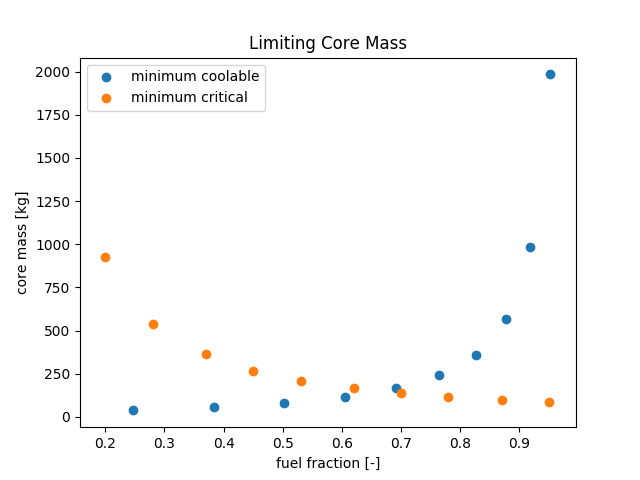
\includegraphics[width=5in]{../images/limiting_core_mass.png}
\caption{Limiting core mass constraints ensure mass-optimized reactor is found.}
\label{fig:limiting_core_mass}
\end{figure}

The reactor configuration calculated by the mass model is the intersection of
the critical core mass and the coolable core mass curves. The critical radius
constraint forced the reactor to be on the critical radius curve. The shape of
both curves ensured the intersection was the minimum mass reactor. For the
critical mass curve, any point below the curve did not meet the target
reactivity and any point above the curve exceeded the target reactivity. For the
coolable mass curve, any point below could not reject the required thermal heat
input and any point above was not reaching its thermal power potential. The
curves have opposite slopes, which means there existed no minimized, valid point on either
curve except for the intersection. Points above both lines represent valid
core designs, but are not the mass-optimized result.


